% Preamble: \

\documentclass{standalone}
\usepackage{pgfplots}
\usepackage{tikz}
\pgfplotsset{width=7cm,compat=1.16}

\begin{document}
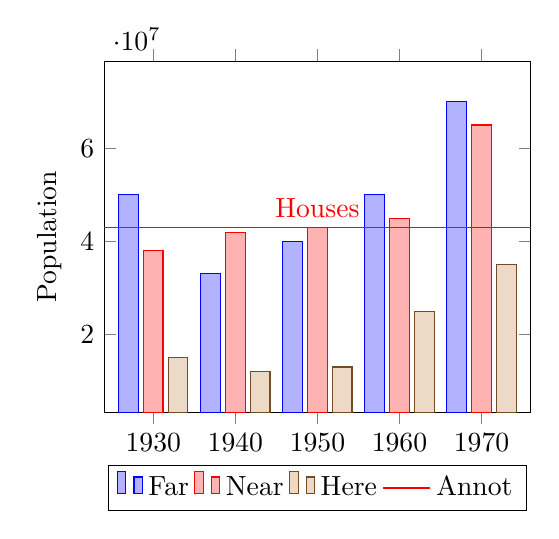
\begin{tikzpicture}
\begin{axis}[
x tick label style={
/pgf/number format/1000 sep=},
ylabel=Population,
enlargelimits=0.15,
legend style={at={(0.5,-0.15)},
anchor=north,legend columns=-1},
ybar,
bar width=7pt,
]
\addplot coordinates {
(1930,50e6) (1940,33e6)
(1950,40e6) (1960,50e6) (1970,70e6)
};
\addplot coordinates {
(1930,38e6) (1940,42e6)
(1950,43e6) (1960,45e6) (1970,65e6)
};
\addplot coordinates {
(1930,15e6) (1940,12e6)
(1950,13e6) (1960,25e6) (1970,35e6)
};
\addplot [red,line legend,
sharp plot,update limits=false,
] coordinates { (1910,4.3e7) (1990,4.3e7) }
node [above] at (1950,4.3e7) {Houses};
\legend{Far,Near,Here,Annot}
\end{axis}
\end{tikzpicture}

\end{document}